% Prof. Dr. Ausberto S. Castro Vera
% UENF - CCT - LCMAT - Curso de Ci\^{e}ncia da Computa\c{c}\~{a}o
% Campos, RJ,  2022
% Disciplina: An\'{a}lise e Projeto de Sistemas
% Aluno: Luiz Miguel Guedes Gomes

\chapterimage{projeto.png} % Table of contents heading image
\chapter{Projeto do Sistema}

Neste capítulo serão apresentadas estratégias para implementação do sistema, assim como diagramas físicos da arquitetura do sistema.

\section{Estrat\'{e}gia do Projeto}

Nessa seção serão apresentadas três tipos de estratégia para a construção do projeto e qual entre elas é mais recomendada.
	
		\subsection{Personalizado}
			Tipo de processo de desenvolvimento de projeto, de forma que este seja criado exclusivamente para a empresa, com intuito de atender necessidades específicas do negócio. Este modelo é recomendado para grandes projetos que abrangem grande numero de detalhes e particularidades, tornando inviável a utilização de soluções prontas.
			Esse tipo de estratégia de construção concede maior liberdade de criação e de solução de problemas do negócio para os desenvolvedores do sistema.
			Recomenda-se fortemente que o sistema Pollinator seja construído baseado neste modelo, devido aos requisitos e necessidades de negócios específicos à esse tipo de empresa e caso seja requisitado um melhor inter-relacionamento entre as partes do sistema e uma maior fluidez de transição entre as interfaces que compõem o projeto.
		\subsection{Software Pronto}
			É o sistema comprado pela empresa já pronto, este deve atender todos os requisitos e necessidades do negócio, visto que nesse tipo de estratégia não deverá ser necessário modificar as especificações e recursos do sistema. Dito isso, conclui-se que esse sistema é melhor recomendado para negócios de pequeno porte com necessidades de negócio e requisitos menos específicos e exigentes.
			Esta estratégia pode ser adotada pelo sistema Pollinator se for feita em conjunto com vários softwares prontos, afim de executar corretamente as sub-funções do sistema. Para isso a integração entre esses sistemas deve ser feita de modo a evitar conflitos e garantir a fluidez de trabalho, e não seria recomendada a utilização dessa estratégia caso o contratante deseje transições menos abruptas entre os sistemas e interfaces que compõem este projeto.
		\subsection{Terceirização}
			Processo onde ocorre a contratação de uma empresa especializada na criação de sistemas para desenvolver o projeto. 
			Para ter êxito nessa estratégia de desenvolvimento, é necessário ter uma documentação bem elaborada, detalhada e precisa, visto que a empresa contratada pode não estar totalmente ciente das diversas realidades do negócio e requisitos discutidos e analisados pelo contratante. Por esses motivos, essa estratégia de desenvolvimento não será adotada para este projeto.


\section{Arquitetura do Sistema - Estilos}
	A seção a seguir utilizará de estilos de arquitetura de sistemas para melhor ilustrar o funcionamento de alguns requisitos e funções do sistema para diferentes visões do projeto: Sobre o sistema, sobre o hardware e sobre o software. 
	

    \subsection{Arquitetura do Sistema}

	\begin{figure}[H]
    \begin{center}
        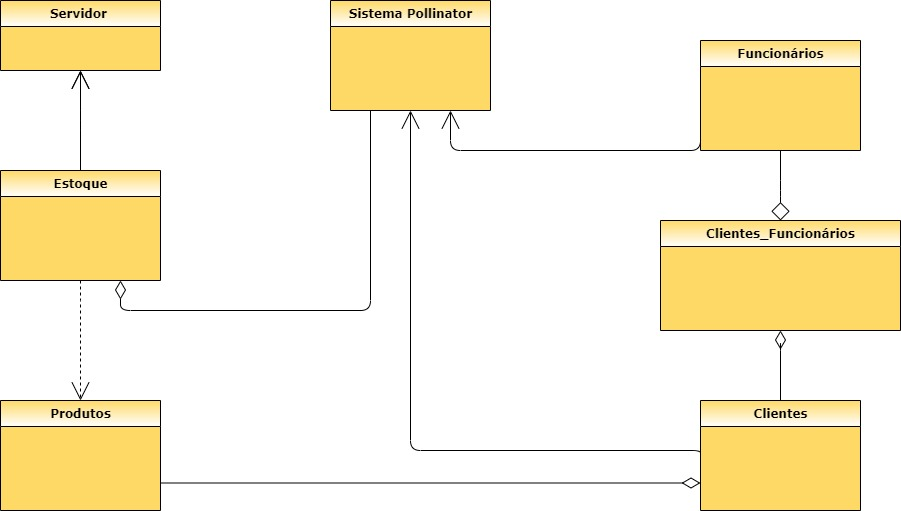
\includegraphics[width=14cm]{Venda_Pollinator_Sistema_Objeto (1).jpg}
        \caption{Diagrama do Sistema de Vendas tipo objeto} \label{sistema}
    \end{center}
   \end{figure} 
   
   \begin{figure}[H]
    \begin{center}
        \includegraphics[width=15cm]{Serviços_Web_Sistema_Servidor.jpg}
        \caption{Diagrama de Sistema de Serviços Web tipo servidor} \label{sistema}
    \end{center}
   \end{figure} 

    \subsection{Arquitetura do Hardware}

	\begin{figure}[H]
    \begin{center}
        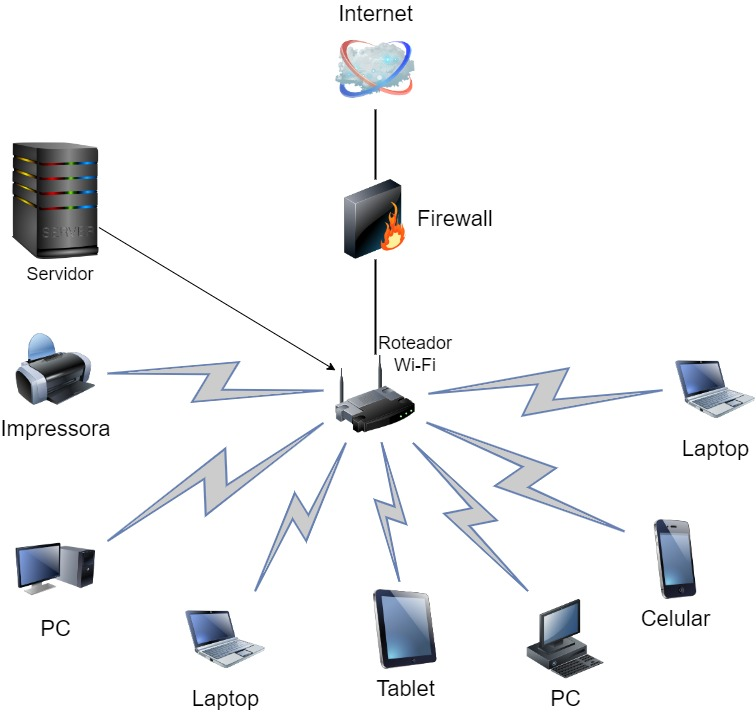
\includegraphics[width=12cm]{Internet_Pollinator_Hardware_Servidor.jpg}
        \caption{Diagrama de Sistema de Internet tipo servidor} \label{sistema}
    \end{center}
   \end{figure} 

	\begin{figure}[H]
    \begin{center}
        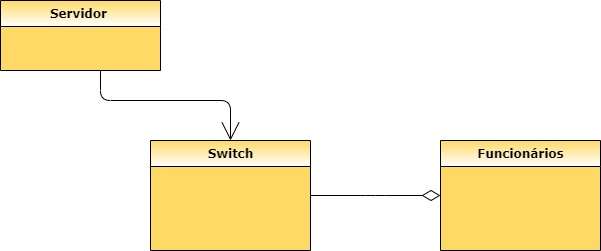
\includegraphics[width=12cm]{Ethernet_Pollinator_Pipe.jpg}
        \caption{Diagrama de Sistema Ethernet tipo pipe} \label{sistema}
    \end{center}
   \end{figure} 

    \subsection{Arquitetura de Software}
	
	\begin{figure}[H]
    \begin{center}
        \includegraphics[width=15cm]{Comentários_Software_Pipe (1).jpg}
        \caption{Diagrama do Sistema de Comentários tipo pipe} \label{sistema}
    \end{center}
   \end{figure} 
   
   \begin{figure}[H]
    \begin{center}
        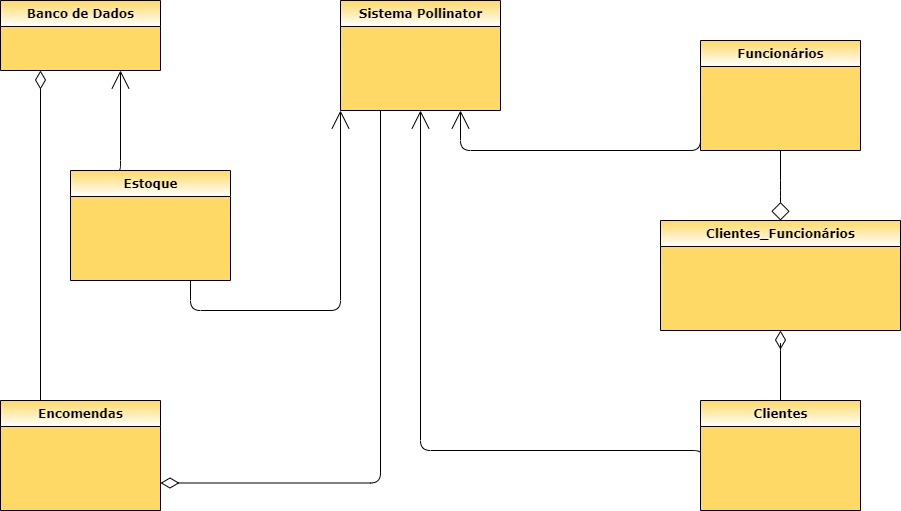
\includegraphics[width=15cm]{Encomendas_Software_Objeto.jpg}
        \caption{Diagrama do Sistema de Encomendas tipo objeto} \label{sistema}
    \end{center}
   \end{figure} 